\documentclass[11pt,a4paper]{article}
\usepackage[utf8]{inputenc}
\usepackage[vietnamese]{babel}
\usepackage{amsmath,amssymb}
\usepackage[version=4]{mhchem}
\usepackage{geometry}
\geometry{top=1.5cm,bottom=1.2cm,left=1.4cm,right=1.4cm,headheight=28pt,headsep=12pt,footskip=18pt}
\usepackage{graphicx}
\usepackage{xcolor}
\usepackage{tabularx}
\usepackage{array}
\usepackage{colortbl}
\usepackage{fancyhdr}
\usepackage{enumitem}

\definecolor{hfRed}{HTML}{D32F2F}
\definecolor{hfGreen}{HTML}{8BC390}
\definecolor{mainGreen}{HTML}{2E7D32}
\definecolor{solBlue}{HTML}{1565C0}
\definecolor{tableGreen}{HTML}{E8F5E9}
\definecolor{ansRed}{HTML}{C62828}

\pagestyle{fancy}
\fancyhf{}
\renewcommand{\headrulewidth}{0.75pt}
\renewcommand{\headrule}{\hbox to\headwidth{\color{hfGreen}\leaders\hrule height \headrulewidth\hfill}}
\renewcommand{\footrulewidth}{0.75pt}
\renewcommand{\footrule}{\hbox to\headwidth{\color{hfGreen}\leaders\hrule height \footrulewidth\hfill}}

\fancyhead[L]{\small\itshape\color{hfRed}Tài liệu lưu hành nội bộ}
\fancyhead[R]{\small\color{hfRed}Thầy \textbf{TRẦN VĂN THẠNH} - 0777.470.803}
\fancyfoot[L]{\footnotesize\itshape\color{hfRed}CS1: 6/15 Nguyễn Hoàng, P. Kim Long, TP Huế \quad | \quad CS2: 24 Đặng Thái Thân, TP Huế}
\fancyfoot[R]{\small\bfseries\color{hfRed}Trang \thepage}

\setlength{\parindent}{0pt}
\setlength{\parskip}{3pt}

\newcommand{\loigiai}[1]{
    \par\vspace{2pt}
    \begingroup\leftskip=12pt
    \textcolor{solBlue}{\textbf{$\blacktriangleright$ Lời giải chi tiết:}}\par
    \small #1
    \par\endgroup\vspace{3pt}
}

\begin{document}


\begin{table}[h!]
\centering
\begin{tabularx}{\textwidth}{@{}p{8.5cm}X@{}}
\textbf{SỞ GIÁO DỤC VÀ ĐÀO TẠO} & \textbf{KIỂM TRA GIỮA HỌC KỲ I} \\
\textbf{ĐỀ CHÍNH THỨC} & \textbf{MÔN: HÓA HỌC - LỚP 12} \\
\textit{(Đề thi có 03 trang)} & Thời gian làm bài: 45 phút \\
\textbf{ } & \textbf{MÃ ĐỀ: 112} \\
\end{tabularx}
\end{table}


\noindent\textit{(Nguyên tử khối trung bình của: H=1, C=12, O=16, N=14, S=32, Na=23, Ag=108, Br=80)}
\par\vspace{-2pt}\noindent\textcolor{gray!40}{\rule{\textwidth}{0.5pt}}\par\vspace{2pt}


\noindent\textbf{\large\color{mainGreen}PHẦN I. (3 điểm) Câu trắc nghiệm nhiều phương án lựa chọn.}\\
\textit{Thí sinh trả lời từ câu 1 đến câu 12. Mỗi câu hỏi thí sinh chỉ chọn một phương án.}
\vspace{4pt}

\textbf{Câu 1.} Chất nào sau đây là ester :\\[2pt]
\begin{tabularx}{\textwidth}{@{}XXXX@{}}\textbf{A.} \ce{CH3COOCH3}. & \textbf{B.} \ce{HCOOH}. & \textbf{C.} \ce{CH3CHO}. & \textbf{D.} \ce{CH3OH}.\end{tabularx}\\[2pt]
\vspace{2pt}
\textbf{Câu 2.} Chất nào sau đây là thành phần chính của chất giặt rửa tổng hợp?\\[2pt]
\begin{tabularx}{\textwidth}{@{}XX@{}}\textbf{A.} \ce{C3H5(OH)3}. & \textbf{B.} \ce{CH3[CH2]14COONa}. \\ \textbf{C.} \ce{CH3[CH2]16COOK}. & \textbf{D.} \ce{CH3[CH2]11C6H4SO3Na}.\end{tabularx}\\[2pt]
\vspace{2pt}
\textbf{Câu 3.} Sodium lauryl sulfate là một trong những chất giặt rửa tổng hợp phổ biến có công thức cấu tạo như sau:\\
\begin{center}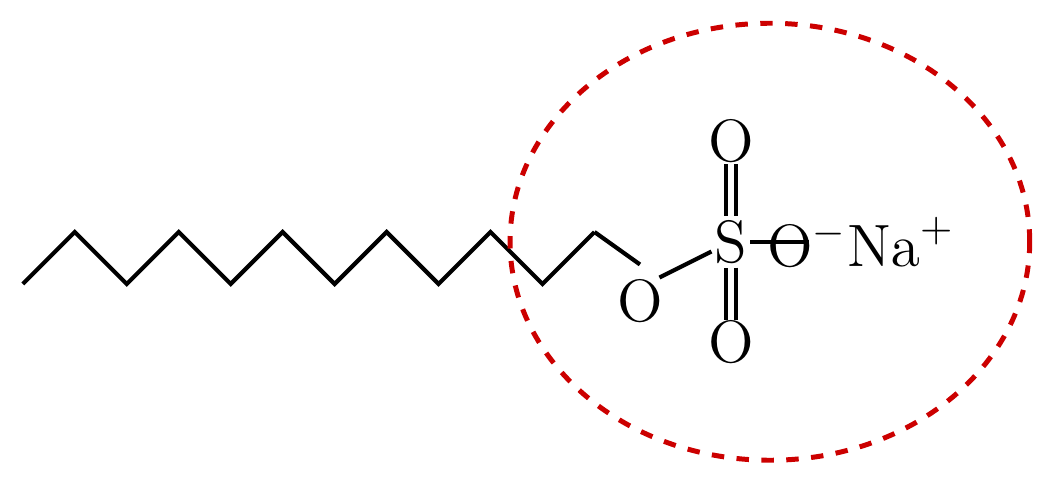
\includegraphics[width=9cm]{images_de112/sodium_lauryl_sulfate.png}\end{center}
Đặc điểm của nhóm được khoanh tròn trong công thức trên là gì?\\[2pt]
\begin{tabularx}{\textwidth}{@{}XX@{}}\textbf{A.} Ưa nước. & \textbf{B.} Tạo kết tủa với nước cứng. \\ \textbf{C.} Không phân cực. & \textbf{D.} Kị nước.\end{tabularx}\\[2pt]
\vspace{2pt}
\textbf{Câu 4.} Cho 6 carbohydrate sau: glucose, fructose, maltose, saccharose, tinh bột và cellulose. Có bao nhiêu carbohydrate đã cho thuộc nhóm monosaccharide ?\\[2pt]
\begin{tabularx}{\textwidth}{@{}XXXX@{}}\textbf{A.} 1 & \textbf{B.} 2 & \textbf{C.} 3 & \textbf{D.} 4\end{tabularx}\\[2pt]
\vspace{2pt}
\textbf{Câu 5.} Saccharose được cấu tạo từ\\[2pt]
\quad \textbf{A.} hai đơn vị $\alpha$-glucose.\\[2pt]
\quad \textbf{B.} một đơn vị $\alpha$-glucose và một đơn vị $\beta$-fructose.\\[2pt]
\quad \textbf{C.} hai đơn vị $\beta$-fructose.\\[2pt]
\quad \textbf{D.} nhiều đơn vị $\alpha$-glucose.\\[2pt]
\vspace{2pt}
\textbf{Câu 6.} Phát biểu nào sau đây đúng khi nói về tinh bột và cellulose?\\[2pt]
\quad \textbf{A.} Đều tham gia phản ứng tráng bạc.\\[2pt]
\quad \textbf{B.} Đều có phản ứng màu với dung dịch iodine.\\[2pt]
\quad \textbf{C.} Đều tan tốt trong nước lạnh.\\[2pt]
\quad \textbf{D.} Thủy phân hoàn toàn trong môi trường acid đều thu được glucose.\\[2pt]
\vspace{2pt}
\textbf{Câu 7.} Cellulose thuộc loại polysaccharide, là thành phần chính tạo nên màng tế bào thực vật, có nhiều trong gỗ, bông nõn. Công thức của cellulose là\\[2pt]
\begin{tabularx}{\textwidth}{@{}XXXX@{}}\textbf{A.} \ce{(C6H10O5)_n}. & \textbf{B.} \ce{C12H22O11}. & \textbf{C.} \ce{C6H12O6}. & \textbf{D.} \ce{C2H4O2}.\end{tabularx}\\[2pt]
\vspace{2pt}
\textbf{Câu 8.} Các amino acid tồn tại chủ yếu ở trạng thái ion lưỡng cực, do đó chúng\\[2pt]
\quad \textbf{A.} có nhiệt độ nóng chảy cao và tan tốt trong nước.\\[2pt]
\quad \textbf{B.} có nhiệt độ nóng chảy cao và ít tan trong nước.\\[2pt]
\quad \textbf{C.} dễ nóng chảy và tan tốt trong nước.\\[2pt]
\quad \textbf{D.} dễ nóng chảy và ít tan trong nước.\\[2pt]
\vspace{2pt}
\textbf{Câu 9.} Glutamic acid có vai trò quan trọng trong quá trình xây dựng cấu trúc tế bào của con người. Glutamic acid có điểm đẳng điện pI = 3,2 (pI là giá trị pH tại đó tổng điện tích trong amino acid bằng không). Khi đặt dung dịch glutamic acid ở pH = 6 trong điện trường, glutamic acid chủ yếu tồn tại ở dạng\\[2pt]
\begin{tabularx}{\textwidth}{@{}XX@{}}\textbf{A.} anion và di chuyển về cực dương. & \textbf{B.} ion lưỡng cực và đứng yên. \\ \textbf{C.} anion và di chuyển về cực âm. & \textbf{D.} cation và di chuyển về cực âm.\end{tabularx}\\[2pt]
\vspace{2pt}
\textbf{Câu 10.} Cho 11,25 gam glycine tác dụng với dung dịch NaOH vừa đủ, cô cạn dung dịch sau phản ứng, thu được m gam muối khan. Giá trị của m là\\[2pt]
\begin{tabularx}{\textwidth}{@{}XXXX@{}}\textbf{A.} 14,55 & \textbf{B.} 13,32. & \textbf{C.} 11,10. & \textbf{D.} 16,65.\end{tabularx}\\[2pt]
\vspace{2pt}
\textbf{Câu 11.} Trong môi trường base, protein có phản ứng màu biuret với\\[2pt]
\begin{tabularx}{\textwidth}{@{}XXXX@{}}\textbf{A.} \ce{HNO3}. & \textbf{B.} \ce{NaCl}. & \textbf{C.} \ce{Cu(OH)2}. & \textbf{D.} \ce{Mg(OH)2}.\end{tabularx}\\[2pt]
\vspace{2pt}
\textbf{Câu 12.} Câu nào sau đây không đúng?\\[2pt]
\quad \textbf{A.} Khi thuỷ phân hoàn toàn protein thu được hỗn hợp các $\alpha$-amino acid.\\[2pt]
\quad \textbf{B.} Có thể sử dụng phản ứng màu biuret để nhận biết sự có mặt của protein.\\[2pt]
\quad \textbf{C.} Protein có thể tạo hợp chất màu vàng khi tác dụng với nitric acid.\\[2pt]
\quad \textbf{D.} Tất cả các loại protein đều không tan trong nước.\\[2pt]
\vspace{2pt}

\vspace{4pt}
\noindent\textbf{\large\color{mainGreen}PHẦN II. (2 điểm) Câu trắc nghiệm đúng sai.}\\
\textit{Trong mỗi ý a), b), c), d) ở mỗi câu, thí sinh chọn đúng hoặc sai.}
\vspace{4pt}

\textbf{Câu 1.} Cho các phát biểu sau:\\[2pt]
\quad \textbf{a)} Glucose và fructose là hai monosaccharide, có công thức phân tử \ce{C6H12O6}.\\[2pt]
\quad \textbf{b)} Trong môi trường acid, glucose và fructose có thể chuyển hóa lẫn nhau.\\[2pt]
\quad \textbf{c)} Dùng dung dịch \ce{AgNO3} trong \ce{NH3} để phân biệt glucose và fructose.\\[2pt]
\quad \textbf{d)} Cho 27 gam glucose lên men thành ethyl alcohol, toàn bộ khí \ce{CO2} sinh ra trong quá trình này được hấp thụ hết vào dung dịch \ce{Ca(OH)2} dư, tạo ra 40 gam kết tủa. Biết hiệu suất quá trình lên men đạt 75\%.\\[2pt]
\vspace{4pt}
\textbf{Câu 2.} Thủy phân hoàn toàn 1 mol peptide X, thu được 1 mol glycine (Gly), 2 mol alanine (Ala), 1 mol valine (Val). Thủy phân không hoàn toàn X thu được tripeptide Gly-Ala-Val và dipeptide Ala-Gly.\\[2pt]

\quad \textbf{a)} X là tetrapeptide, có 3 liên kết peptide.\\[2pt]
\quad \textbf{b)} X hòa tan \ce{Cu(OH)2} trong môi trường kiềm tạo dung dịch màu xanh lam.\\[2pt]
\quad \textbf{c)} Peptide X luôn có amino acid đầu N là Ala, amino acid đầu C của X là Val.\\[2pt]
\quad \textbf{d)} Thủy phân hoàn toàn 31,6 gam X bằng dung dịch NaOH dư, thu được 45,8 gam muối. Mặt khác thủy phân hoàn toàn 31,6 gam X bằng dung dịch HCl dư, thu được 51,6 gam muối.\\[2pt]

\vspace{4pt}
\noindent\textbf{\large\color{mainGreen}PHẦN III. (2 điểm) Câu trắc nghiệm yêu cầu trả lời ngắn.}\\
\textit{Thí sinh trả lời từ câu 1 đến câu 4.}
\vspace{4pt}

\textbf{Câu 1.} Cho các chất: \ce{CH3[CH2]14COONa}, \ce{CH3[CH2]10CH2OSO3Na}, \ce{CH3[CH2]16COOK}, \ce{CH3[CH2]7CH=CH[CH2]7COONa}, \ce{CH3COONa}, \ce{(C15H31COO)3C3H5}. Có bao nhiêu chất có thể là thành phần chính của xà phòng?\\[2pt]
\textbf{Trả lời:} \dotfill\\[4pt]
\vspace{2pt}
\textbf{Câu 2.} Thủy phân hoàn toàn 4,34 gam tripeptide mạch hở X (được tạo nên từ hai $\alpha$-amino acid có công thức dạng \ce{H2NC_x H_y COOH}) bằng dung dịch NaOH dư, thu được 6,38 gam muối. Mặt khác thủy phân hoàn toàn 4,34 gam X bằng dung dịch HCl dư, thu được bao nhiêu gam muối? (làm tròn đến hàng phần trăm)\\[2pt]
\textbf{Trả lời:} \dotfill\\[4pt]
\vspace{2pt}
\textbf{Câu 3.} Củ sắn khô chứa 38\% khối lượng là tinh bột, còn lại là các chất không có khả năng lên men thành ancol etylic. Lên men 1 tấn sắn khô với hiệu suất cả quá trình là 81\%. Toàn bộ lượng ancol etylic sinh ra để điều chế xăng E5 (có chứa 5\% thể tích ancol etylic). Biết khối lượng riêng của ancol etylic là 0,8 g/mL, thể tích xăng E5 thu được là bao nhiêu lít? ( làm tròn đến hàng đơn vị)\\[2pt]
\textbf{Trả lời:} \dotfill\\[4pt]
\vspace{2pt}
\textbf{Câu 4.} Cho các nhận định sau:\\
(1) Protein dạng hình cầu và dạng hình sợi tan tốt trong nước.\\
(2) Một trong những tính chất hoá học đặc trưng của protein là phản ứng thuỷ phân.\\
(3) Phản ứng của protein với nitric acid cho sản phẩm có màu tím.\\
(4) Khi đun nóng lòng trắng trứng sẽ xảy ra hiện tượng đông tụ.\\
(5) Trong cơ thể, enzyme đóng vai trò là chất xúc tác sinh học.\\
Liệt kê các nhận định đúng theo dãy số thứ tự tăng dần ( Ví dụ: 1234, 134, 24...)\\[2pt]
\textbf{Trả lời:} \dotfill\\[4pt]
\vspace{2pt}

\vspace{4pt}
\noindent\textbf{\large\color{mainGreen}PHẦN IV. Tự luận (3,0 điểm)}\\
\textit{Thí sinh trình bày chi tiết lời giải các câu hỏi sau:}
\vspace{4pt}

Câu 1 (1,0 điểm). Viết tất cả các công thức cấu tạo của amine có công thức phân tử \ce{C3H9N}? Gọi tên thay thế?\\[2pt]
\par\noindent\dotfill\\
\noindent\dotfill\\
\noindent\dotfill\\
\noindent\dotfill\\
\noindent\dotfill\\[4pt]
\vspace{2pt}
Câu 2 (1,0 điểm). Nêu hiện tượng, viết phương trình phản ứng khi cho:\\
a) Saccharose phản ứng với \ce{Cu(OH)2} ở nhiệt độ thường.\\
b) Dẫn methylamine vào dung dịch muối \ce{FeCl3}.\\[2pt]
\par\noindent\dotfill\\
\noindent\dotfill\\
\noindent\dotfill\\
\noindent\dotfill\\
\noindent\dotfill\\[4pt]
\vspace{2pt}
Câu 3 (1,0 điểm).\\
a) Cho dãy các chất: phenyl acetate, allyl acetate, methyl acetate, ethyl formate, tripalmitin. Có bao nhiêu chất trong dãy khi thủy phân trong dung dịch NaOH (dư), đun nóng sinh ra alcohol ? Viết phương trình phản ứng?\\
b) Aspirin là một hợp chất được sử dụng làm giảm đau, hạ sốt được điều chế theo phản ứng sau:\\
\ce{(CH3CO)2O + HOC6H4COOH -> CH3COOC6H4COOH + CH3COOH}\\
Để sản xuất 500 nghìn viên thuốc aspirin cần tối thiểu m kg salicylic acid. Biết rằng mỗi viên thuốc có chứa 81 mg aspirin và hiệu suất phản ứng đạt 75\%. Giá trị của m là bao nhiêu?\\[2pt]
\par\noindent\dotfill\\
\noindent\dotfill\\
\noindent\dotfill\\
\noindent\dotfill\\
\noindent\dotfill\\[4pt]
\vspace{2pt}

\begin{center}
\textbf{---------- HẾT ----------}
\end{center}
\end{document}
